\chapter*{Appendix} \label{appendix}

\begin{figure}[!h]
\centering 
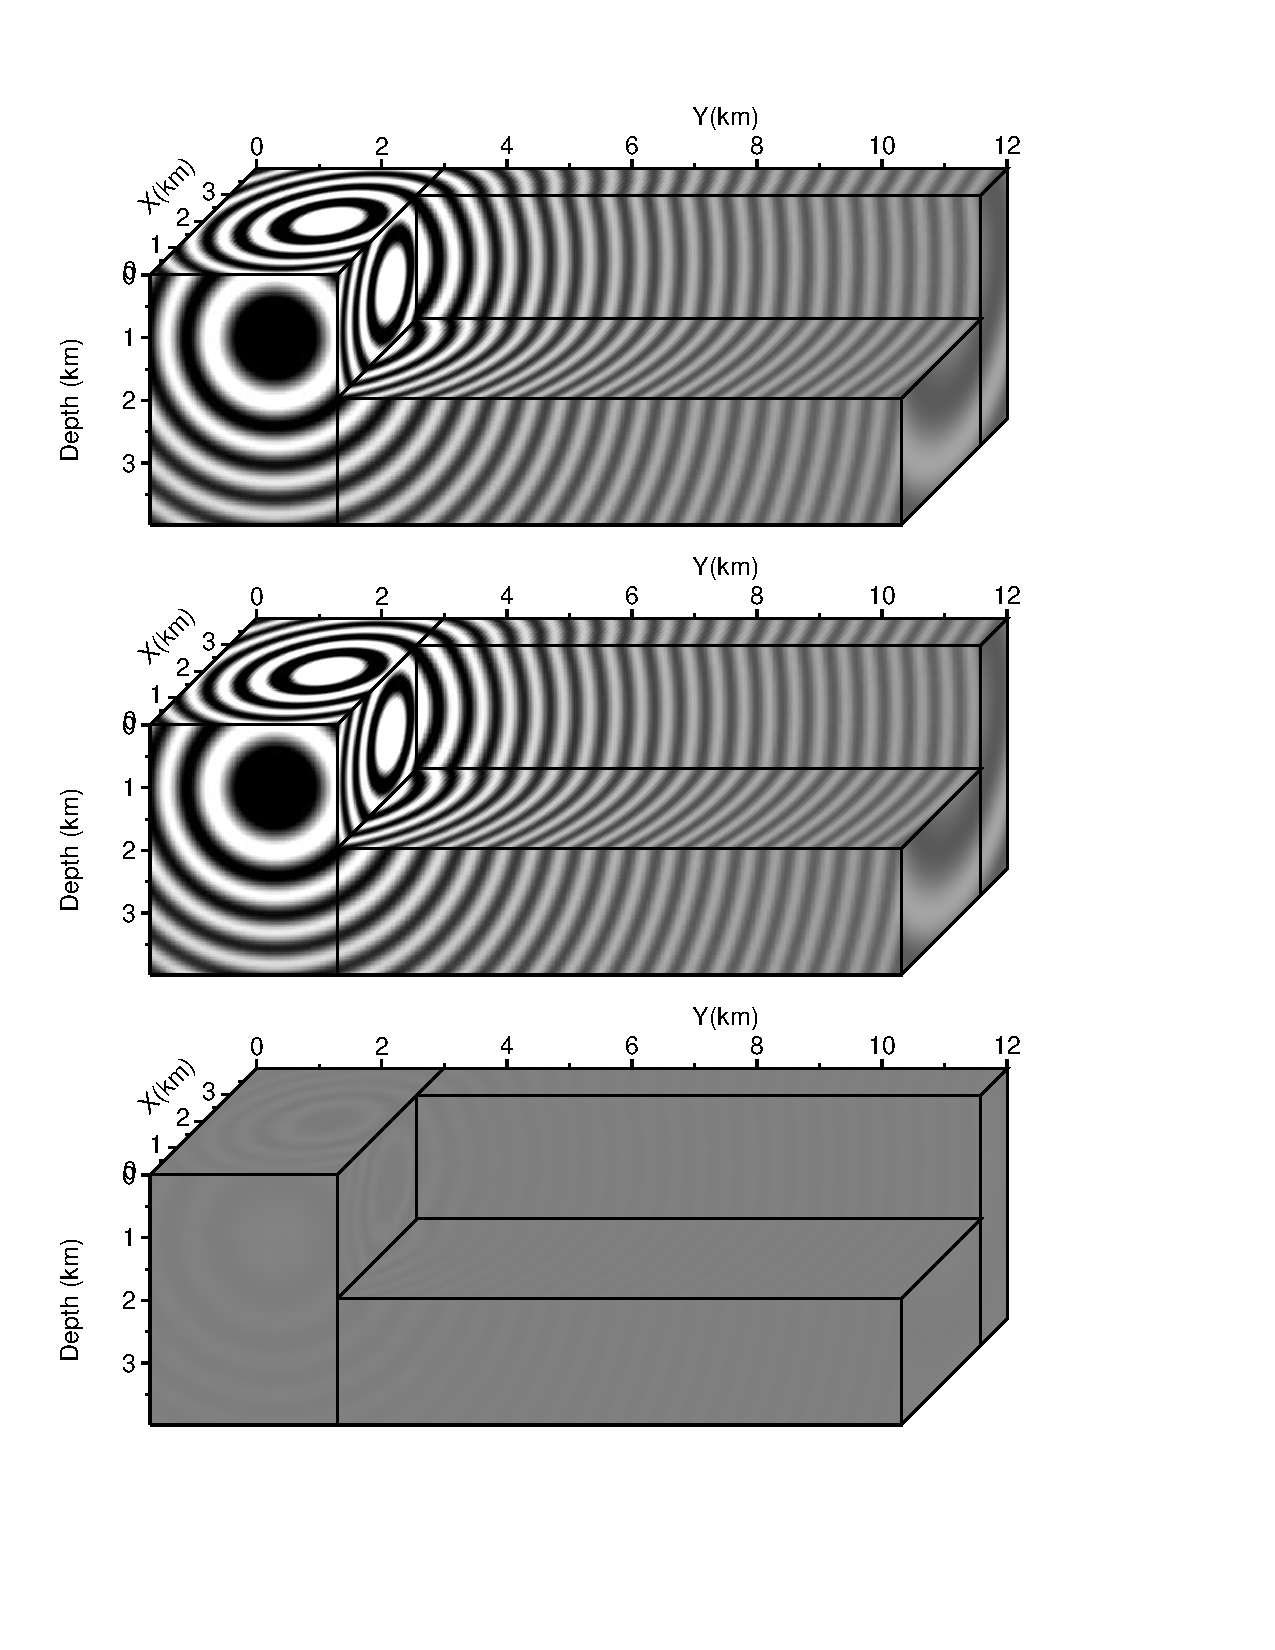
\includegraphics[width=0.75\textwidth]{images/dsfdm/fig_cube_homogeneous_isotropic.pdf}
\caption{Bench Homogeneous Isotropic. Infinite homogeneous isotropic medium. Validation against analytical solution. a) DSFDM solution. b) Analytical solution. c) Difference.}
\label{cube_homogeneous_isotropic} 
\end{figure}
\begin{figure}[!h]
\centering 
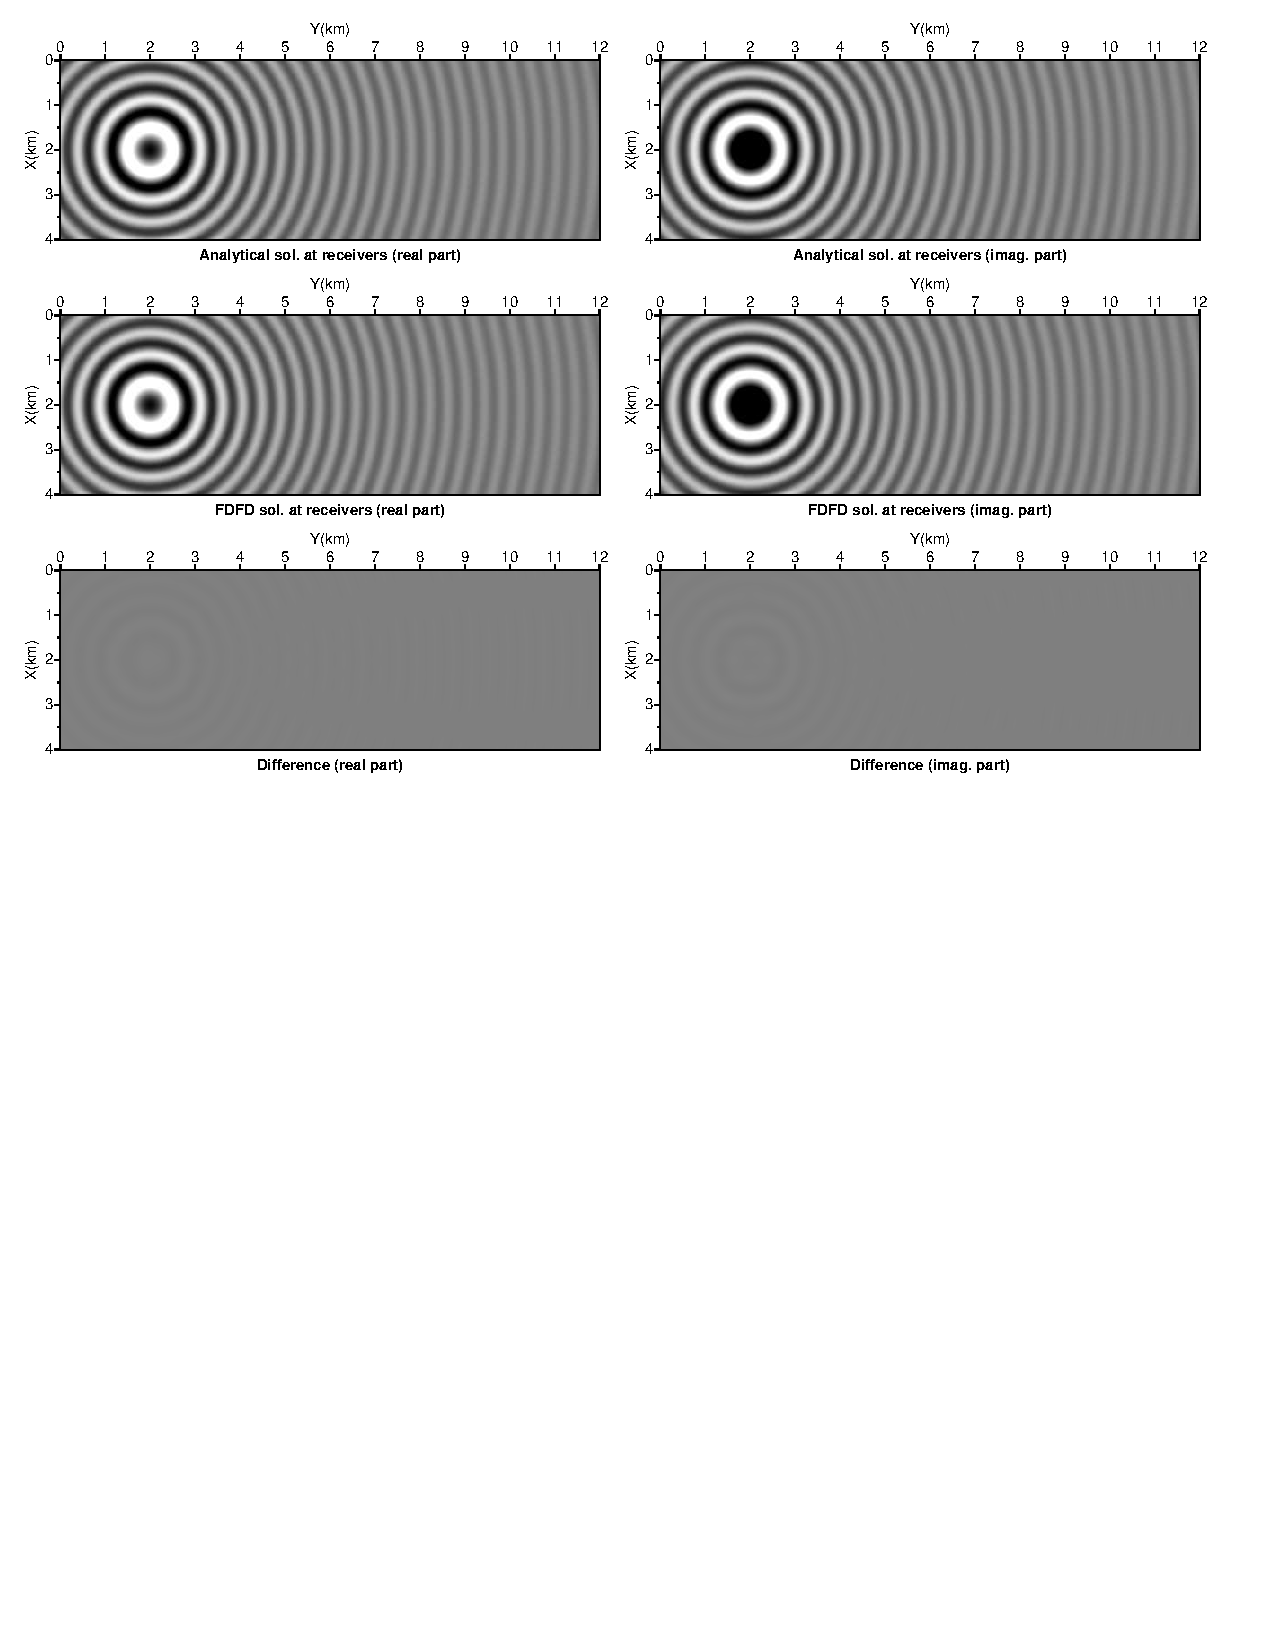
\includegraphics[width=0.75\textwidth]{images/dsfdm/fig_rec_snap_homogeneous_isotropic.pdf}
\caption{Bench Homogeneous Isotropic. Infinite homogeneous isotropic medium. Validation against analytical
solution. Solution at receiver positions, 1km below the surface.}
\label{rec_snap_homogeneous_isotropic} 
\end{figure}
\begin{figure}[!h]
\centering 
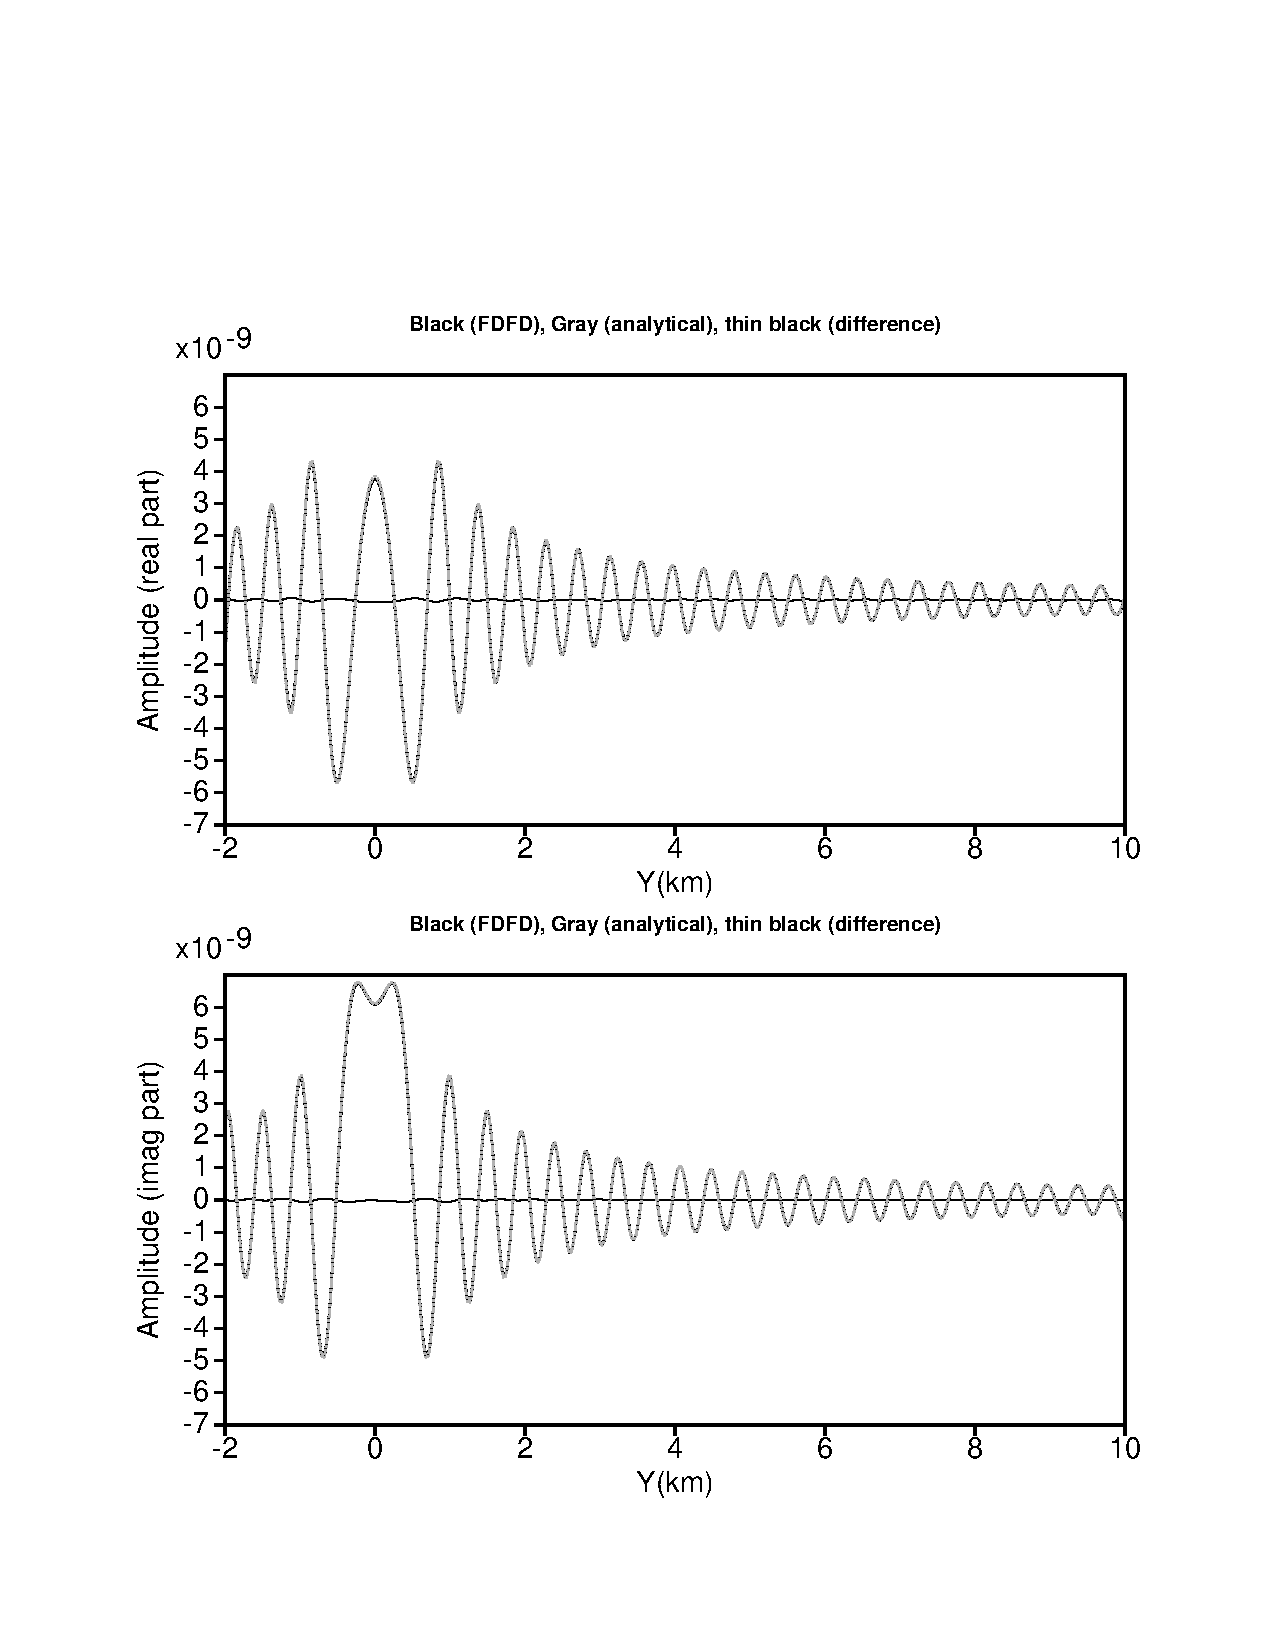
\includegraphics[width=0.75\textwidth]{images/dsfdm/fig_rec_log_homogeneous_isotropic.pdf}
\caption{Bench Homogeneous Isotropic. Infinite homogeneous isotropic medium. Validation against analytical
solution. Solution at receiver positions along the Y profile running across the shot position.}
\label{rec_log_homogeneous_isotropic} 
\end{figure}


\begin{figure}[!h]
\centering 
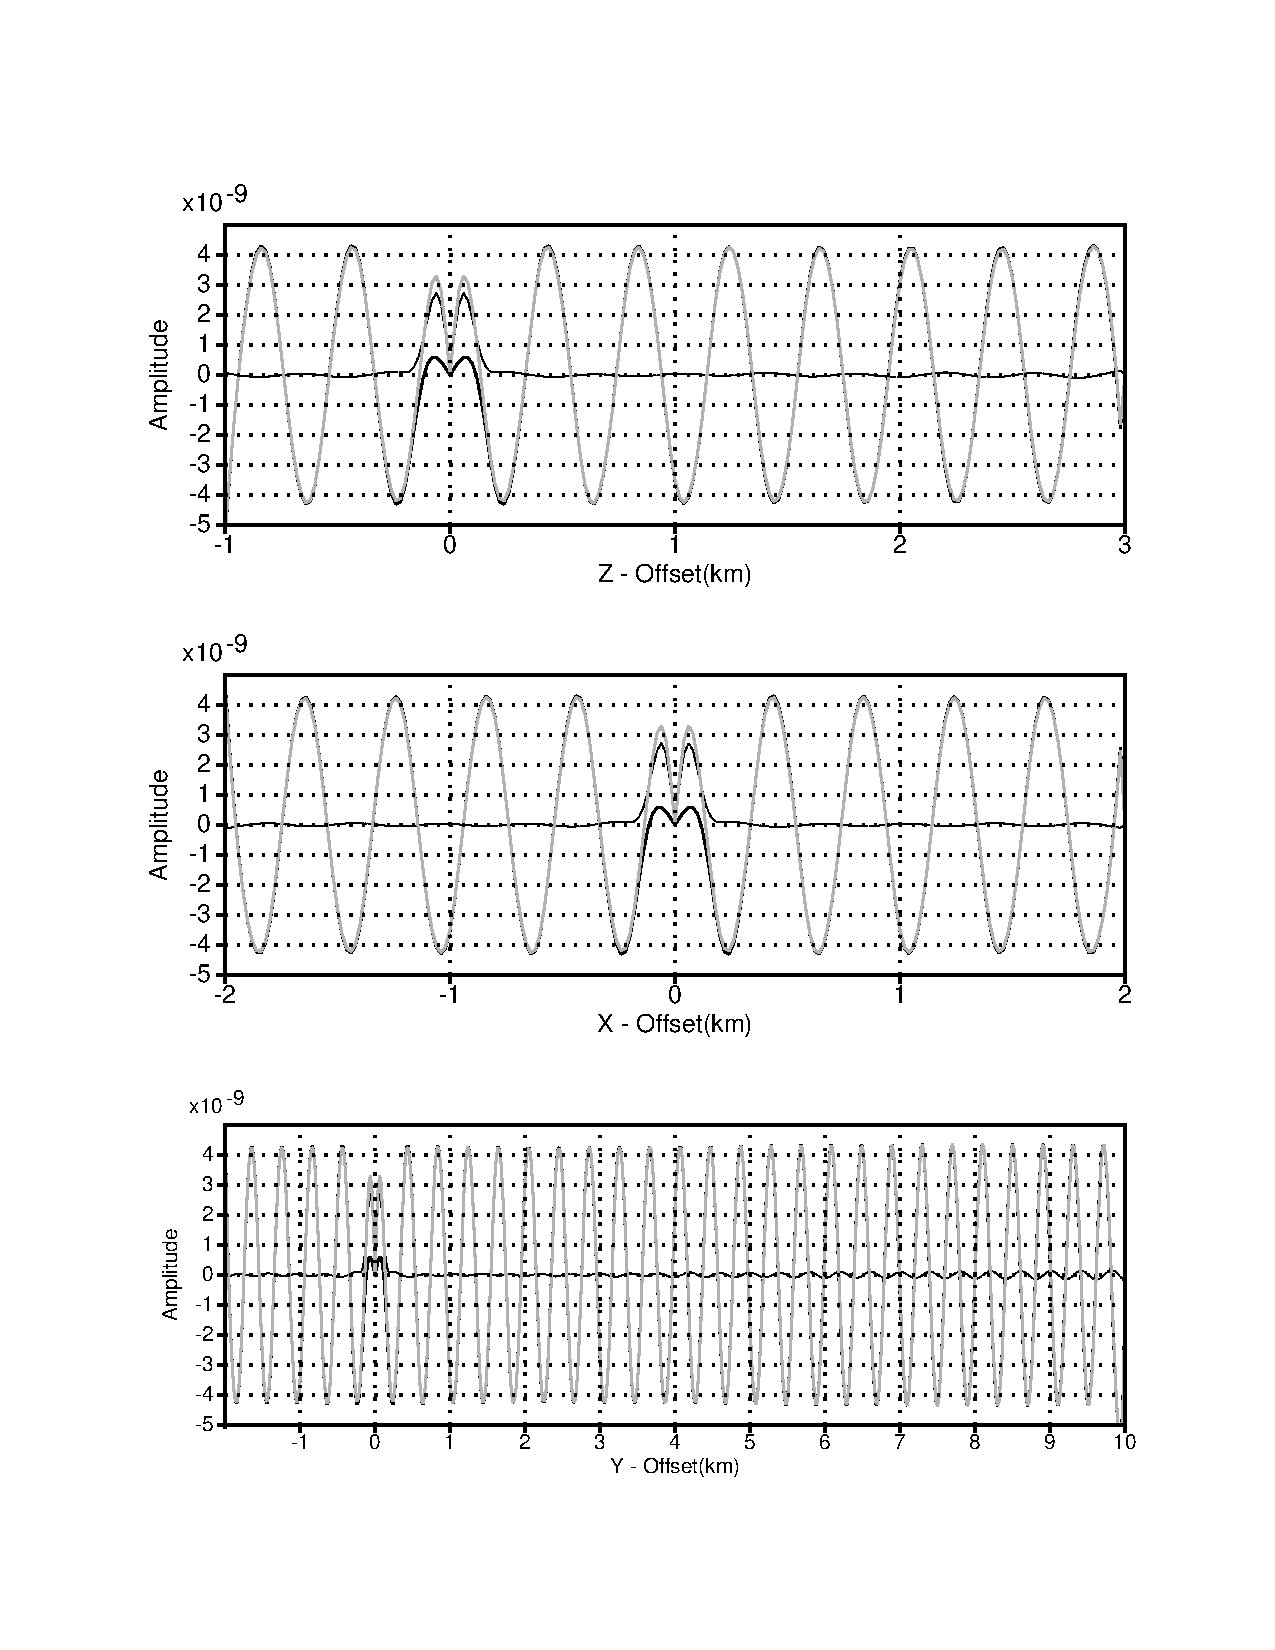
\includegraphics[width=0.75\textwidth]{images/dsfdm/fig1_log_homogeneous_isotropic.pdf}
\caption{Bench Homogeneous Isotropic. Infinite homogeneous isotropic medium. Validation against analytical
solution. Logs across shot position with correction for geometrical spreading.}
\label{fig1_log_homogeneous_isotropic} 
\end{figure}
\begin{figure}[!h]
\centering 
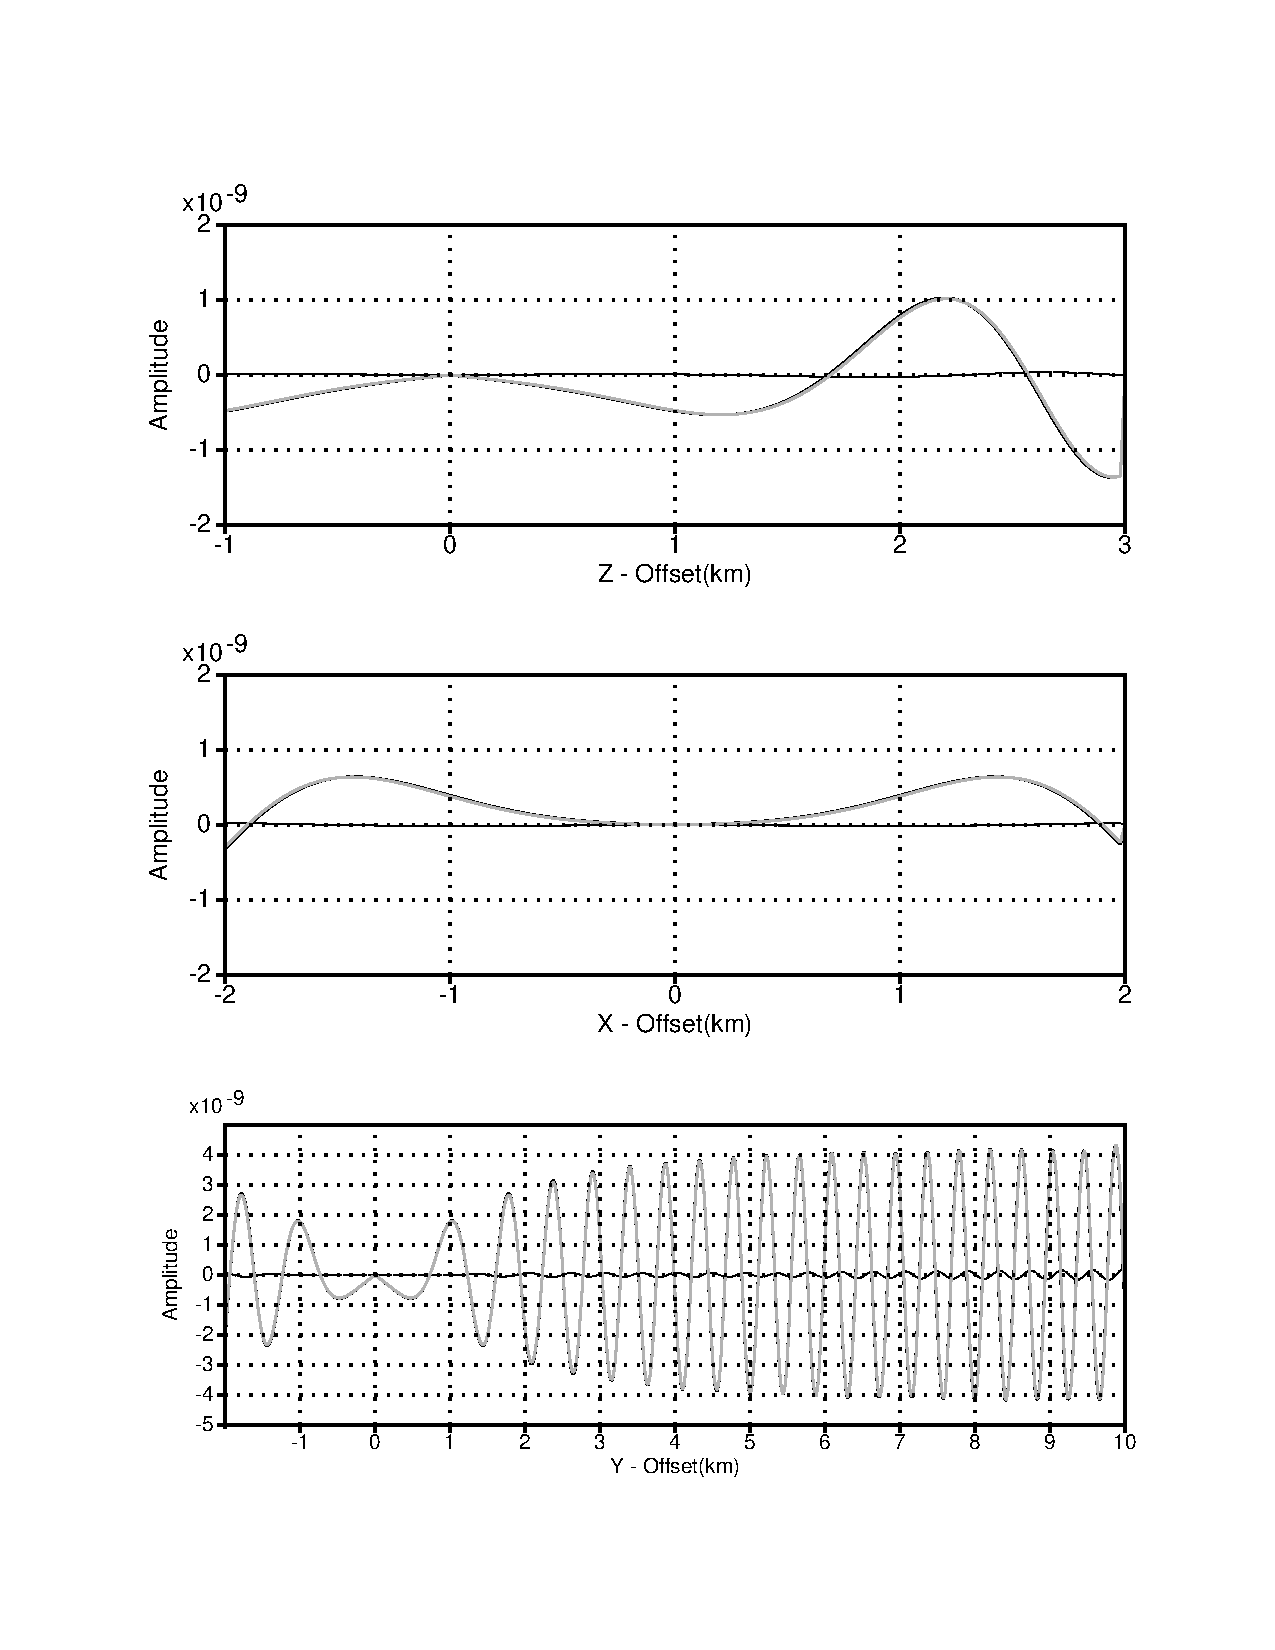
\includegraphics[width=0.75\textwidth]{images/dsfdm/fig2_log_homogeneous_isotropic.pdf}
\caption{Bench Homogeneous Isotropic. Infinite homogeneous isotropic medium. Validation against analytical
solution. Logs along the slices of Fig. ??b with correction for geometrical spreading.}
\label{fig2_log_homogeneous_isotropic} 
\end{figure}

\begin{figure}[!h]
\centering 
  \begin{subfigure}[b]{0.7\textwidth}
    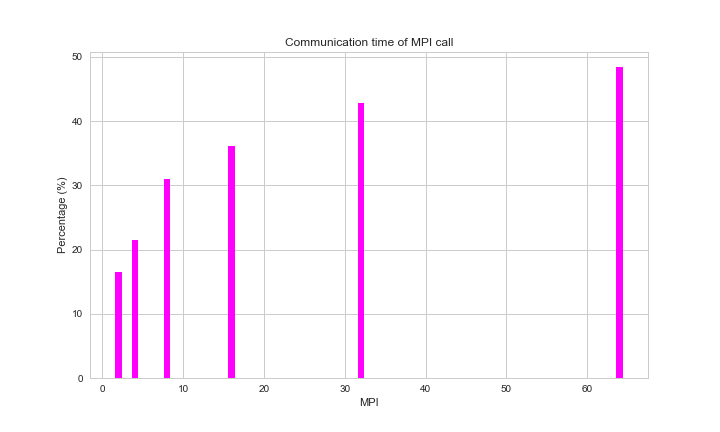
\includegraphics[width=\textwidth]{images/MPIProfInca.png}
    \caption{Communication time of MPI call in classical nodes}
    \label{MPIProfInca}
  \end{subfigure}
  %
  \begin{subfigure}[b]{0.7\textwidth}
    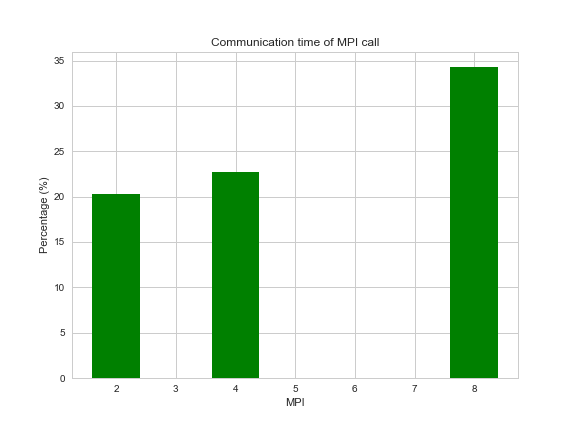
\includegraphics[width=\textwidth]{images/MPIProfMesc.png}
    \caption{Communication time of MPI call in Mesca node}
    \label{MPIProfMesc}    
  \end{subfigure}
  \caption{Comparison of Communication time of MPI call between Mesca and classical nodes}
\end{figure} 
\begin{figure}[!h]
\centering 
  \begin{subfigure}[b]{0.7\textwidth}
    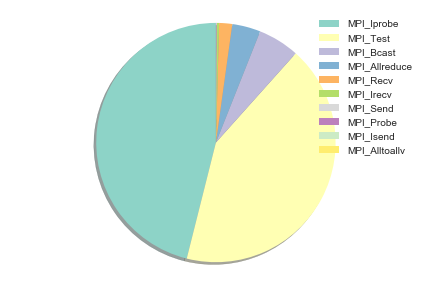
\includegraphics[width=\textwidth]{images/PieInca2process.png}
    \caption{MPI call in classical nodes where number of process 2}
    \label{MPIProfInca}
  \end{subfigure}
  %
  \begin{subfigure}[b]{0.7\textwidth}
    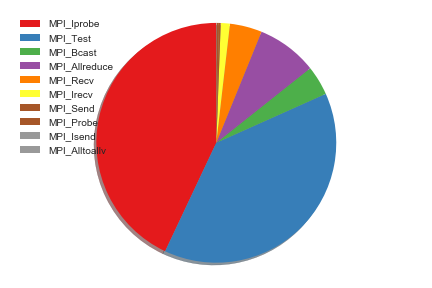
\includegraphics[width=\textwidth]{images/PieMesca2process.png}
    \caption{MPI call in classical nodes where number of process 2}
    \label{MPIProfMesc}
  \end{subfigure}
  \caption{Comparison MPI call between Mesca and classical nodes where number of process 2}
\end{figure}

\begin{figure}[!h]
\centering 
  \begin{subfigure}[b]{0.7\textwidth}
    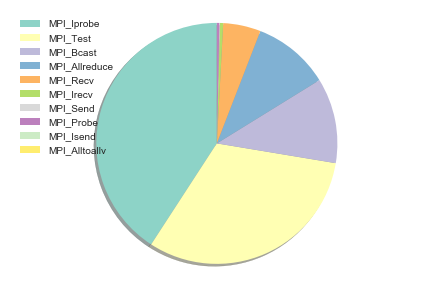
\includegraphics[width=\textwidth]{images/PieInca4process.png}
    \caption{MPI call in classical nodes where number of process 4}
    \label{MPIProfInca}
  \end{subfigure}
  %
  \begin{subfigure}[b]{0.7\textwidth}
    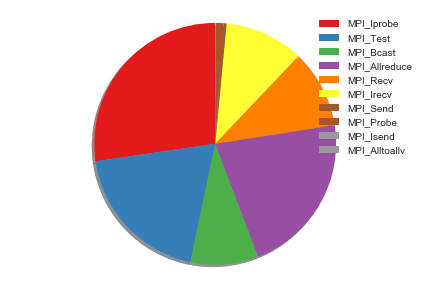
\includegraphics[width=\textwidth]{images/PieMesca4process.png}
    \caption{MPI call in classical nodes where number of process 4}
    \label{MPIProfMesc}
  \end{subfigure}
  \caption{Comparison MPI call between Mesca and classical nodes where number of process 4}
\end{figure}

\begin{figure}[!h]
\centering 
  \begin{subfigure}[b]{0.7\textwidth}
    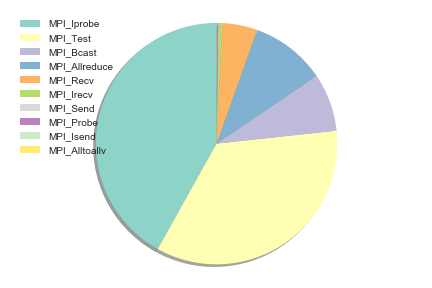
\includegraphics[width=\textwidth]{images/PieInca8process.png}
    \caption{MPI call in classical nodes where number of process 8}
    \label{MPIProfInca}
  \end{subfigure}
  %
  \begin{subfigure}[b]{0.7\textwidth}
    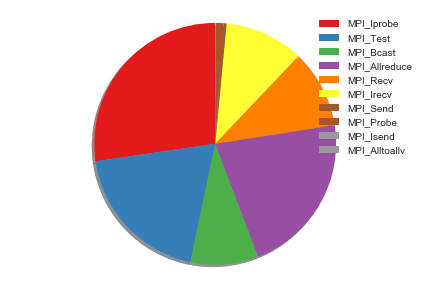
\includegraphics[width=\textwidth]{images/PieMesca4process.png}
    \caption{MPI call in classical nodes where number of process 4}
    \label{MPIProfMesc}
  \end{subfigure}
  \caption{Comparison MPI call between Mesca and classical nodes where number of process 8}
\end{figure}